\documentclass{cpsc413Solutions}
\usepackage{amsmath}
\usepackage[utf8]{inputenc}
\usepackage{graphicx}
\graphicspath{{Images/}}
\usepackage{ dsfont }
\usepackage{ upgreek }
\usepackage{listings}


\coursetitle{Design and Analysis of Algorithms}
\courselabel{CPSC 413}
\exercisesheet{Problem Set \#[6]}{}
\student{Minh Hang Chu - 30074056}
\semester{Winter 2020}

\begin{document}

\team{Minh Hang Chu}

\sources{
Lecture Notes,
Algorithm Design textbook
}

\begin{problemlist}
\pbitem 
\begin{problem}
\begin{answer}

We can skip this question.

\end{answer}

\newpage

\pbitem
\begin{problem}
\begin{answer}

\begin{enumerate}
    \item Give a formal definition (pre- and post-conditions) of the problem described.
    
    Pre-condition:
    \begin{itemize}
        \item A $n \times n $ checkerboard, like a matrix that has index: bottom left is (1,1), top left is (1,n), bottom right is (n,0) and top right (n,n).
        
        We define $C = \{1,2,3 \dots n\} \times \{1,2,3, \dots, n\}$ to be the coordinates of the squares in the checkerboard.
        
        \item A cost function $p: C \times C \xrightarrow{} \mathds{R}$ that is the amount of money to travel to go from square $x$ to $y$.
    \end{itemize}
    Post-conditions:
    \begin{itemize}
        \item A starting point $s=(x,1), 1\leq x \leq n$.
        \item An ending point $f=(1,y), 1 \leq y \leq n$
        \item output set of moves $M = [m_1, \dots m_k]$ where each element of $M$ is an arrow, denotes going up left 1, going up straight 1 and going up right 1 $\nwarrow, \uparrow, \nearrow $. Each moves in $M$ corresponds to the valid move $\{ (-1,1),(0,1),(1,1)\}$.
        \item All moves in $M$ must be valid, makes sure not going off the board.
        \item The cost of set of moves $M$ is maximum when reaching the ending point.
        \item outputs the maximum value $p$.

    \end{itemize}
    
\newpage
    \item Describe the optimal substructure relationship for this problem by giving expression $d[i,j]$.
    
    Let's start from $(i,j)$, we will work backward to reach some square at row 0.
    
    We have 3 different possible moves: 
    
    \begin{itemize}
        \item The square immediately below
        \item The square that is one down to the left (but only if the checker is not already in the leftmost column)
        \item The square that is one down to the right (but only if the checker is not already in the rightmost column)
    \end{itemize}
    
    Thus, the optimal substructure relationship is:
    
    
    \begin{align*}
    d[i,j] = 
        \begin{cases}
        0   &\text{if $j=1$}\\
        \\
        \max\{p((i,j-1), (i,j))+d[i,j-1],\\
               p((i-1,j-1), (i,j))+ d[i-1,j-1] & \text{if $i=n$}\\
               \\
        \max\{p((i,j-1), (i,j))+d[i,j-1],\\
               p((i+1,j-1), (i,j))+d[i+1,j-1]\} & \text{if $x=1$}\\
               \\
        \max\{p((i,j-1), (i,j))+d[i,j-1],\\
               p((i-1,j-1), (i,j))+ d[i-1,j-1],\\
               p((i+1,j-1), (i,j))+d[i+1,j-1]\} & \text{otherwise}
        \end{cases}
    \end{align*}
    
    \newpage
    
    \item Pseudocode for recursive algorithm and non-recursive driver program\\
    
    Recursive algorithm:
    
    \begin{lstlisting}[numbers=left, mathescape=true]
maxValue($i,j$){
    if ($j==1$){  // at the bottom of board
        return 0
    }
    else if ($i==1$){ // at leftmost square of the board
        $dm = p((i,j-1), (i,j))+maxValue(i,j-1)$
        $dr = p((i+1,j-1), (i,j))+maxValue(i+1,j-1)$
        return $\max(dm,dr)$
    }
    else if ($j==n$){ // at rightmost square of the board
        $dm = p((i,j-1), (i,j))+maxValue(i,j-1)$
        $dl = p((i-1,j-1), (i,j))+maxValue(i-1,j-1)$
        return $\max(dm,dl)$
    }
    else{
        $dm = p((i,j-1), (i,j))+maxValue(i,j-1)$
        $dl = p((i-1,j-1), (i,j))+maxValue(i-1,j-1)$
        $dr = p((i+1,j-1), (i,j))+maxValue(i+1,j-1)$
        return $\max(dm,dl,dr)$
    }
}
\end{lstlisting}

The non-recursive driver program:

\begin{lstlisting}[numbers=left, mathescape=true]
driver{
    result = $-\infty$
    for $i=0$ to $n-1$
        result = $\max(result, maxValue(i,n-1))$
    end for
    return result
}
\end{lstlisting}
    
    \newpage
    \item Recurrence relation representing an upper bound of recursive algorithm.
    
    It's obvious to see the worst case recurrence relation:
    
    \begin{align*}
    T[i,j] = 
        \begin{cases}
         c  &\text{if $j=1$}\\
        \\
       T(i,j-1)+T(i+1,j-1)+T(i-1,j-1) + d & \text{otherwise}
        \end{cases}
    \end{align*}
    
    We simplify this as:
    $T(i,j) = T(n)$
    \begin{align*}
    T[i,j] = 
        \begin{cases}
         c  &\text{if $j=1$}\\
        \\
       T(n-1)+T(n-1)+T(n-1) + d & \text{otherwise}
        \end{cases}
    \end{align*}
    
    which means:
    \begin{align*}
    T[i,j] = 
        \begin{cases}
         c  &\text{if $j=1$}\\
        \\
       3T(n-1) + d & \text{otherwise}
        \end{cases}
    \end{align*}
    
    \newpage
    \item State and prove asymptotic upper bound
    
    We have the tree below:
    \begin{figure}[htp]
        \centering
        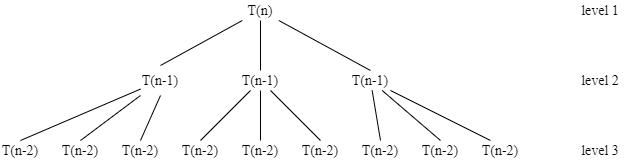
\includegraphics[width=15cm]{ProbSet6.png}
    \end{figure}
    
    At level 1, the total cost is $d$.\\
    At level 2, the total cost is $3d = 3^{2-1}d$.\\
    At level 3, the total cost is $9d = 3^P{3-1}d$.\\
    
    We see the pattern, at level $h$ the total cost is $3^{h-1}d$. 
    
    The tree has the same height, our guess for recurrence is:
    
    $$\sum_{i=1}^{n} 3^{i-1}d = d \sum_{i=1}^n3^{i-1}= d \sum_{i=1}^{n-1}3^{i}= d \frac{3^{N}-1}{3-1} = \frac{d}{2}(3^N-1)$$
    
    Our guess is the recurrence is in $O(\frac{d}{2}(3^n-1))$.
    
    We prove this induction.
    
    Choose $n_0 = 1$.
    Base case: $n = 1$\\
    Then $T(n) = T(1) =c$. Let $a \geq \frac{2c}{d}$. We have $c\leq a \leq a\frac{d}{2}(3-1)$. We are done for base case.

    Inductive Hypothesis: For $k \in \mathds{Z}, k \geq 1, T(k) \leq a\frac{d}{2}(3^{k}-1)$.
    
    Inductive Step: We want to show $T(n+1) < a\frac{d}{2}(3^k-1)$.
    
    We have: 
    $$T(k+1) = 3T(k) +d \leq 3(a\frac{d}{2}(3^k-1) + d \leq \frac{ad}{2}3^{k+1} - \frac{3ad}{2} +d$$
    
    We want to add $\frac{-ad}{2} - (\frac{-3ad}{2}+d)$ to the expression to get $a\frac{d}{2}(3^{k+1}-1)$.
    
    Choose $a = max{1,\frac{2c}{d}}$, we will get
    
    $$T(k+1) \leq \frac{ad}{2}3^{k+1} - \frac{3ad}{2}+d \leq \frac{ad}{2}3^{k+1}-\frac{ad}{2} = a\frac{d}{2}(3^{k+1}-1)$$.
    
    Hence, $T(n) \in O(\frac{d}{2}(3^n-1)$ which is in $O(3^n)$.
    
    Hence, $T(n) \in O(3^n)$.
    
    \newpage
    \item Pseudocode for dynamic programming
    
    \begin{lstlisting}[numbers=left, mathescape=true]
maxCheckerBoardValues() {
    $C = n\times n$  // initialize
    $M = n\times n$  // initialize
    for $i = 1..n$ 
        for $j = 1..n$ 
            if $(j == 1)$
                $C[i,j] = 0$
            else if $(i == 1)$ { // at leftmost column
                $dm = p((i,j-1), (i,j)) + C[i, j- 1]$
                $dr =  p((i + 1,j-1), (i,j)) + C[i + 1, j-1]$
                $C[i,j] = max(dm, dr)$
                if $C[i,j] == dm$
                    $M[i, j] = \downarrow$
                else if $C[i,j] == dr$
                    $M[i,j] = \searrow$
            else if $(i == n)$ // at the rightmost column
                $dm = p((i,j-1), (i,j)) + C[i, j- 1]$
                $dl =  p((i - 1,j-1), (i,j)) + C[i - 1, j- 1]$
                $C[i,j] = max(dm, dl)$
                if $C[i,j] == dm$
                    $M[i, j] = \downarrow$
                else if $C[i,j] == dl$
                    $M[i, j] = \swarrow$
            else
                $dm = p((i,j-1), (i,j)) + C[i, j- 1]$
                $dl =  p((i - 1,j-1), (i,j)) + C[i - 1, j- 1]$
                $dr =  p((i + 1,j-1), (i,j)) + C[i + 1, j- 1]$
                $C[i,j] = max(dm, dl, dr)$
                if $C[i,j] == dm$
                    $M[i, j] = \downarrow$
                else if $C[i,j] == dr$
                    $M[i,j] = \searrow$
                else if $C[i,j] == dl$
                    $M[i,j] = \swarrow$
            end if
        end for
    end for
// Trace back to get set of moves
Move = []
checkerBoardRecover($C,M$) {
    // find the max ending position
    $maxCost = -\infty$
    for $i = 1 \dots n$
        if $C[i,n] \geq maxCost$
            maxCost = C[i,n]
            (i,j) = (i,n)
        end if
    end for
    while (j != 1) 
        if ($M[i,j] == \downarrow$)
            $Moves.add(\uparrow)$
            $j = j -1$
        else if $M[i,j] == \searrow$ 
            $Moves.add(\nwarrow)$
            $i = i + 1$
            $j = j - 1$
        else if $M[i,j] == \swarrow$ 
            $Moves.add(\nearrow)$
            $i = i - 1$
            $j = j - 1$
        end if 
    end while
    return $Moves, s = (i,j), maxCost$
end
\end{lstlisting}
    
    \newpage 
    \item State and prove tight asymptotic bound for dynamic programming algorithm.
    
    Tight aymptotic bound on the run time for the algorithm is $O(n^2)$
    
    \begin{itemize}
        \item Initialization step take $\Theta(n^2)$.
        \item From line 4, we have nested for loop. Look at the loop inside which goes from 1 to n. Inside the loop takes constant time $c_1$. Hence, the run time of the inner for loop in $nc_1$.
        \item The outer for loop also runs from 1 to n, each iteration takes $nc_1$ time. Hence, the total run time of this nestet for loop is $n^2c_1$ which is in $\Theta(n^2)$.
        \item At line 42, to find the maximum end position. We use loop to find the maxCost and ending position. The loop body takes constant time $c_2$ and iterates from 1 to n. Hence,the runtime for this loop is $\Theta(n)$.
        \item The next loop body also takes constant time. The loop iterates through from the maximum to the starting point which is also in $\Theta(n)$
        \item Finally we return the list which takes constant time.
        \item Hence, put everything together, we have $$\Theta(n^2) + \Theta(n^2) + \Theta(1) +\Theta(n) +\Theta(n) \in \Theta(n^2) $$.
    \end{itemize}
    Thus, the tight asymptotic bound is $Theta(n^2)$.
\end{enumerate}
\end{answer}
\end{problem}
\end{problem}

\end{problemlist}

\end{document}
